\documentclass{a4beamer}
%% Lectures - common definitions

\usextensions{tikz}
\usetikzlibrary{shapes.multipart,shapes.callouts,shapes.geometric}
\input{fix-callouts.inc} % Fixes absolute positioning of rectangle callouts

\newif\ifbigpages \bigpagesfalse
\ifdim\paperwidth >20cm
	\bigpagestrue
\fi

\tikzset{%
	note/.style={rectangle callout,draw=none,callout pointer width=1em,%
		align=flush left,font=\footnotesize,inner sep=0.5em,%
		fill=blue!15,fill opacity=0.95,text opacity=1.0,callout absolute pointer=#1},
	node distance=2em and 2.75em
}
\ifbigpages
	% Scale all arrow tips by the factor of 2.5
	\let\old@pgf@arrow@call=\pgf@arrow@call
	\def\pgf@arrow@call#1{%
		\@tempdima=\pgflinewidth%
		\pgfsetlinewidth{2.5\pgflinewidth}%
		\old@pgf@arrow@call{#1}%
		\pgfsetlinewidth{\@tempdima}%
	}
	\def\pgfarrowsleftextend#1{\pgfmathsetlength{\pgf@xa}{1.5*#1}}
	\def\pgfarrowsrightextend#1{\pgfmathsetlength{\pgf@xb}{1.5*#1}}
\fi

%% Load listings package
\usepackage{listings}

%% Are we inside a comment?
\newif\iflstcomment \lstcommentfalse

\lstset{%
	tabsize=4,
	showstringspaces=false,
	basicstyle=\linespread{1.25}\ttfamily\small,
	keywordstyle=\bfseries,
	commentstyle=\lstcommentstyle,
	numbers=left,
	numberstyle=\footnotesize\color{gray},
	xleftmargin=2.5em,
	extendedchars=true,
	escapechar=\$,
	escapebegin=\iflstcomment\begingroup\lstcommentstyle\fi,
	escapeend=\iflstcomment\endgroup\fi
}

\def\lstcommentstyle{\color{gray}}

\lst@AddToHook{AfterBeginComment}{\global\lstcommenttrue}
\let\orig@lst@EndComment=\lst@EndComment
\def\lst@EndComment{\global\lstcommentfalse\orig@lst@EndComment}
\lst@AddToHookAtTop{EOL}{%
	\lst@ifLmode\global\lstcommentfalse\fi% XXX Sloppy way to determine comment end
}

%% Python with docstrings treated as comments
\lstdefinelanguage[doc]{python}[]{python}{%
	deletestring=[s]{"""}{"""},%
	morecomment=[s]{"""}{"""}%
}%

%% JavaScript language
\lstdefinelanguage{javascript}%
	{morekeywords={break,case,catch,%
		const,constructor,continue,default,do,else,false,%
		finally,for,function,if,in,instanceof,%
		new,null,prototype,%
		return,switch,this,throw,%
		true,try,typeof,var,while},%
	sensitive,%
	morecomment=[l]//,%
	morecomment=[s]{/*}{*/},%
	morestring=[b]",%
	morestring=[b]',%
}[keywords,comments,strings]%

%% C# language (4.0?)
\lstdefinelanguage{csharp}%
	{morekeywords={abstract,as,%
		base,bool,byte,case,catch,char,%
		checked,class,const,continue,%
		decimal,default,delegate,do,double,%
		else,enum,event,explicit,extern,%
		false,finally,fixed,float,for,foreach,%
		goto,if,implicit,in,int,interface,%
		internal,is,lock,long,%
		namespace,new,null,object,operator,out,%
		override,params,private,protected,public,%
		readonly,ref,return,sbyte,sealed,%
		short,sizeof,stackalloc,static,string,%
		struct,switch,this,throw,true,try,%
		typeof,uint,ulong,unchecked,unsafe,ushort,%
		using,virtual,void,volatile,while%
	},%
	sensitive,%
	morecomment=[l]//,%
	morecomment=[s]{/*}{*/},%
	morestring=[b]",%
	morestring=[b]',%
}[keywords,comments,strings]%

%% Translation for fact environment
\deftranslation[to=russian]{Fact}{Наблюдение}

%% Inline code snippets
\def\code#1{\texttt{#1}}
\def\codekw#1{\code{\textbf{#1}}}

\def\quoteauthor#1{\par\footnotesize\upshape\hfill—~#1}

%% English term
\def\engterm#1{(англ. \textit{#1})}
%% Term with explanation below (to be used in diagrams)
\def\termwithexpl#1#2{#1\strut{}\\\small\color{gray}(\textit{#2})\strut{}}
%% External link
\def\extlink#1#2{\href{#1}{\color[rgb]{0.7,0.7,1.0}\dashbar{#2}}}
%% Internal link
\def\inlink#1#2{\hyperlink{#1}{\color[rgb]{0.7,0.7,1.0}\dashbar{#2}}}
%% Explanation for a list item
\def\itemexpl#1{\begingroup\small\vspace{0.75ex}#1\par\endgroup}



\usetikzlibrary{shapes.misc}


\lecturetitle{Программная инженерия. Лекция №14 — Верификация и валидация}
\title[V \& V]{Верификация и валидация}
\author{Алексей Островский}
\institute{\small{Физико-технический учебно-научный центр НАН Украины}\vspace{2ex}}
\date{12 марта 2015 г.}

\def\hoaretri#1#2#3{%
	\{#1\}\ #2\ \{#3\}%
}

\begin{document}
	\frame{\titlepage}

	\section{Введение}

	\subsection[Определение]{Определение верификации и валидации}

	\frame{
		\frametitle{Верификация и валидация}

		\begin{Definition}
			\textbf{Верификация} \engterm{verification} — процессы проверки соответствия программного продукта 
			требованиям и спецификациям, заданным при его проектировании.
		\end{Definition}

		\vspace{1ex}
		\begin{Definition}
			\textbf{Валидация} \engterm{validation} — процессы проверки соответствия программного продукта 
			потребностям заказчика; проверка корректности спецификаций.
		\end{Definition}

		\vspace{1ex}
		\begin{center}
			\begin{tabular}{|p{0.2\textwidth}|p{0.325\textwidth}|p{0.325\textwidth}|}
				\hline
				& Верификация & Валидация \cr
				\hline
				\textbf{Цель} & \raggedright Правильно ли строится~ПП? & \raggedright Строится ли правильный~ПП? \cr
				\hline
				\textbf{Точка зрения} & \raggedright разработчик (белый ящик) & \raggedright конечный пользователь (черный ящик) \cr
				\hline
				\textbf{Методы} & статические & \raggedright динамические (тестирование) \cr
				\hline
			\end{tabular}
		\end{center}
	}

	\subsection{Методы верификации}

	\frame{
		\frametitle{Методы верификации}

		\textbf{Неформальные методы:}
		\begin{itemize}
			\item инспекции и обзоры кода; 
			\item инструменты для автоматического поиска ошибок в коде.
		\end{itemize}

		\vspace{1ex}
		\textbf{Формальные методы верификации:} 
		\begin{itemize}
			\item проверка моделей ПО \engterm{model checking}; 
			\item (автоматизированные) доказательства корректности программ; 
			\item абстрактная интерпретация кода; 
			\item системы типов данных.
		\end{itemize}
	}

	\subsection{Необходимость верификации}

	\frame{
		\frametitle{Необходимость верификации}

		\begin{center}
			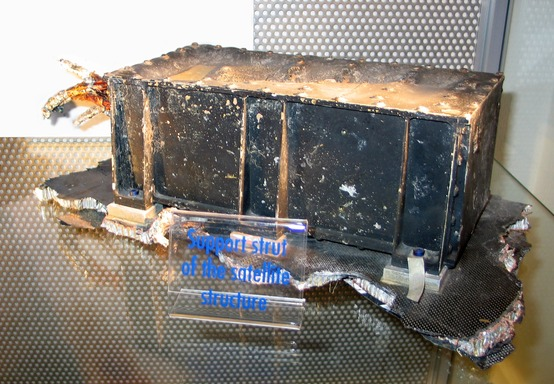
\includegraphics[height=0.7\textheight]{fig-Ariane.jpg}
		\end{center}

		\figureexpl{%
			Фрагмент спутника \extlink{http://en.wikipedia.org/wiki/Cluster_\%28spacecraft\%29}{«Ariane 5»}, 
			потерпевшего крушение в~1996~г. 
			Причиной аварии стало преобразование из~64-битного числа с~плавающей запятой в~16-битное целое без~должной проверки, 
			что~привело к~переполнению и~аппаратному исключению. 
			Цена ошибки составила $\sim$350 млн.~\$.}
	}

	\frame{
		\frametitle{Необходимость верификации}

		\begin{center}
			\begin{tikz*}[%
	every node/.style={align=center}
]
	\node(arrow-st) [coordinate] {};
	\node(arrow-tip) [coordinate,right=30em of arrow-st] {};

	\node(testing-c) [coordinate,right=7.5em of arrow-st] {};
	\node(testing) [above=0.5em of testing-c] {Тестирование};
	\node(analysis-c) [coordinate,right=15em of arrow-st] {};
	\node(analysis) [above=0.5em of analysis-c] {Анализ кода};
	\node(formal-c) [coordinate,right=22.5em of arrow-st] {};
	\node(formal) [above=0.5em of formal-c] {Формальные \\ методы};

	\node(speed) [below=0.5em of arrow-st] {Скорость};
	\node(complete) [below=0.5em of arrow-tip] {Полнота};

	\draw[->] (arrow-st) -- (arrow-tip);
	\draw (testing-c) ++(0,0.5em) -- ++(0,-1em);
	\draw (analysis-c) ++(0,0.5em) -- ++(0,-1em);
	\draw (formal-c) ++(0,0.5em) -- ++(0,-1em);
\end{tikz*}

		\end{center}

		\vspace{1ex}
		\textbf{Область применения верификации:}
		\begin{itemize}
			\item
			критические системы, системы реального времени (напр., системы управления спутниками и~ракетами);
			\item
			системы с высокими требованиями к надежности / отказоустойчивости (напр., системы шифрования);
			\item
			ПО, регулируемое нормативными документами (напр., ПО, использующееся в~медицине).
		\end{itemize}
	}

	\section{Инспекции}

	\frame{
		\frametitle{Инспекции}

		\begin{Definition}
			\textbf{Инспекции кода} \engterm{code inspections} — анализ кода программы 
			или ее абстрактного представления (напр., UML диаграммы) человеком на предмет наличия ошибок.
		\end{Definition}

		\vspace{1ex}
		\begin{center}
			{\small\begin{tikz*}[%
	every node/.style={rectangle,draw,align=center,minimum height=3.25em}
]
	\node(spec) {Спецификация \\ требований};
	\node(arch) [right=of spec] {Архитектура ПО};
	\node(uml) [right=of arch] {Модели UML};
	\node(schema) [right=of uml] {Схемы БД};
	\node(program) [right=of schema] {Программы};
	\node(proto) [below=of spec] {Прототипы \\ системы};

	\node(inspect) [rounded rectangle,above=of uml] {Инспекции};
	\node(testing) [rounded rectangle] at (uml.south |- proto.west) {Тестирование};

	\draw[->] (spec) -- (proto);
	\draw[->] (testing) -- (proto);
	\draw[->] (testing) -| (program);

	\node(_tmp) [coordinate] at ($ (inspect.south)!0.5!(uml.north) $) {};
	\draw (inspect) -- (_tmp);
	\draw[->] (_tmp) -| (spec);
	\draw[->] (_tmp) -| (arch);
	\draw[->] (_tmp) -- (uml);
	\draw[->] (_tmp) -| (schema);
	\draw[->] (_tmp) -| (program);
\end{tikz*}
}

			\figureexpl{Возможности инспекций шире, чем тестирования}
		\end{center}
	}

	\subsection{Преимущества инспекций}

	\frame{
		\frametitle{Преимущества инспекций}

		\begin{itemize}
			\item
			\textbf{Отсутствие взаимодействия} между дефектами (в~отличие от~тестирования, где~одна~ошибка может скрывать другие).

			\vspace{1ex}
			\item
			Возможность \textbf{проверки неполных версий} системы без~дополнительных затрат.

			\vspace{1ex}
			\item
			\textbf{Проверка свойств} программы (соответствие стандартам, портируемость, легкость поддержки).

			\vspace{1ex}
			\item
			Выявление \textbf{неэффективных / неподходящих алгоритмов}.
		\end{itemize}
	}

	\subsection{Области проверки кода}

	\frame{
		\frametitle{Области проверки кода}

		\begin{itemize}
			\item
			\textbf{Дефекты данных:}
			\begin{itemize}
				\item инициализация переменных перед использованием; 
				\item отсутствие «магических» констант; 
				\item индексация элементов массивов / списков; 
				\item потенциальные случаи переполнения буфера.
			\end{itemize}

			\vspace{1ex}
			\item
			\textbf{Дефекты выполнения:} 
			\begin{itemize}
				\item проверка условий ветвления; 
				\item конечность циклов; 
				\item корректность блоков операций; 
				\item полнота вариантов и наличие \textbf{break} в операторе \textbf{switch} / \textbf{case}.
			\end{itemize}

			\vspace{1ex}
			\item
			\textbf{Дефекты ввода/вывода:} 
			\begin{itemize}
				\item использование всех входных переменных; 
				\item присвоение выходных переменных.
			\end{itemize}
		\end{itemize}
	}

	\frame{
		\frametitle{Области проверки кода}

		\begin{itemize}
			\item
			\textbf{Дефекты интерфейсов:}
			\begin{itemize}
				\item корректное количество и порядок аргументов при вызове функций / методов; 
				\item соответствие ожидаемых и фактических типов аргументов; 
				\item идентичность структуры разделяемой памяти.
			\end{itemize}

			\vspace{1ex}
			\item
			\textbf{Дефекты работы с памятью:} 
			\begin{itemize}
				\item корректность работы со связанными объектами (изменение всех требуемых ссылок); 
				\item корректность выделения / освобождения памяти.
			\end{itemize}

			\vspace{1ex}
			\item
			\textbf{Дефекты обработки исключений:} 
			\begin{itemize}
				\item полнота проверок возникновения исключительных ситуаций.
			\end{itemize}
		\end{itemize}
	}

	\subsection{Парное программирование}

	\frame{
		\frametitle{Парное программирование}

		\begin{Definition}
			\textbf{Парное программирование} \engterm{pair programming} — способ разработки~ПО, 
			при~котором код, написанный первым программистом, немедленно проверяется вторым программистом; 
			альтернатива формальным инспекциям в гибкой методологии разработки.
		\end{Definition}

		\vspace{1.5ex}
		\textbf{Достоинства:} более глубокое понимание кода — обнаружение большего числа дефектов.

		\vspace{1ex}
		\textbf{Недостатки:} 
		\begin{itemize}
			\item повышенный шанс непонимания требований; 
			\item пропуск ошибок из-за высокого темпа разработки; 
			\item необъективность инспектора.
		\end{itemize}
	}

	\subsection{Автоматизация}

	\frame{
		\frametitle{Автоматизация инспекций}

		\textbf{Инструменты автоматизации инспекций:}
		\begin{itemize}
			\item
			\textbf{среды разработки} — встроенные средства или~плагины для~проведения инспекций 
			и~неформальных обзоров кода;

			\vspace{1ex}
			\item
			\textbf{системы контроля версий} (Subversion, git, …) — упрощение доступа к~коду, 
			запросы на~изменение / уточнение фрагментов программ;

			\vspace{1ex}
			\item
			\textbf{Lint} — семейство программ статического анализа кода для:
			\begin{itemize}
				\item поиска типичных ошибок, 
				\item устранения непортируемых / потенциально опасных конструкций;
				\item соблюдения принятого стиля написания программного кода.
			\end{itemize}
		\end{itemize}
	}

	\section{Формальные методы}

	\frame{
		\frametitle{Формальные методы}

		\begin{Definition}
			\textbf{Формальные методы} в разработке ПО — методы спецификации, разработки и~верификации~ПО 
			на~основе строгих математических моделей.
		\end{Definition}

		\vspace{1ex}
		\textbf{Уровни использования:}
		\begin{enumerate}
			\item создание формальной модели;
			\item разработка и верификация на основе мат. моделей;
			\item формальное доказательство свойств ПО.
		\end{enumerate}
	}

	\frame{
		\frametitle{Типы формальных методов}

		\begin{center}
			Формальный метод $\simeq$ семантика ЯП.
		\end{center}

		\begin{itemize}
			\item
			\textbf{Денотационная семантика} — подход к программе как функции, преобразующей входные данные в~выходные.

			\vspace{0.5ex}
			\textbf{Примеры:} используется в академической среде (функциональные ЯП).

			\vspace{1ex}
			\item
			\textbf{Аксиоматическая семантика} — подход к программе как к набору пред- и~постусловий для~каждого выполненного действия.

			\vspace{0.5ex}
			\textbf{Примеры:} логика Хоара, языки спецификации.

			\vspace{1ex}
			\item
			\textbf{Операционная семантика} — подход к программе как последовательности действий в~определенной модели.

			\vspace{0.5ex}
			\textbf{Примеры:} проверка моделей, абстрактная интерпретация, символьное выполнение.
		\end{itemize}
	}

	\subsection{Логика Хоара}

	\frame{
		\frametitle{Логика Хоара}

		\begin{Definition}
			\textbf{Функциональная корректность алгоритма} — соответствие выходных данных ожидаемым для~каждой комбинации входных данных.
		\end{Definition}

		\vspace{1ex}
		\begin{Definition}
			\textbf{Полная корректность} — алгоритм корректен и~выполняется за~конечное время для~любого входа.
		\end{Definition}

		\vspace{1ex}
		\begin{Definition}
			\textbf{Логика Хоара} \engterm{Hoare logic} — набор правил вывода для~доказательства 
			функциональной корректности компьютерных программ, записанных с~помощью императивного языка программирования.
		\end{Definition}

		\vspace{1.5ex}
		\figureexpl{(Существует расширение логики Хоара для доказательства полной корректности.)}
	}

	\frame{
		\frametitle{Правила вывода в логике Хоара}

		\textbf{Утверждения — тройки Хоара:}
		\[ \hoaretri{P}{C}{Q}; \]
		$C$ — команда языка программирования; \\
		$P$ — предусловие (предикат, истинный до выполнения команды $C$); \\
		$Q$ — постусловие (предикат, истинный после выполнения команды $C$).

		\vspace{2ex}
		\textbf{Правила вывода (общий вид):}
		\[ T_1 \vdash T_2; \]
		\vspace{-3ex}
		\begin{itemize}
			\item из утверждений $T_1$ выводятся утверждения $T_2$;
			\item ($\Leftrightarrow$) для доказательства $T_2$ достаточно доказать $T_1$.
		\end{itemize}
	}

	\frame{
		\frametitle{Правила вывода в логике Хоара}

		\begin{enumerate}
			\item
			\textbf{Аксиома пропуска:} $\vdash \hoaretri{P}{\mathbf{skip}}{P}$.

			\vspace{2ex}
			\item
			\textbf{Аксиома присвоения:} $\vdash \hoaretri{P[E/x]}{x := E}{P}$, \\
			$P[E/x]$ — замена всех вхождений выражения~$x$ в~предикате~$P$ на~$E$.

			\vspace{1ex}
			\textbf{Пример:} $\vdash \hoaretri{x+1 \leq 5}{x:= x + 1}{x \leq 5}$.

			\vspace{2ex}
			\item
			\textbf{Правило композиции:} $\hoaretri{P}{S}{Q}, \hoaretri{Q}{T}{R} \vdash \hoaretri{P}{S; T}{R}$.

			\vspace{1ex}
			\textbf{Пример:} 
			\begin{multline*}
				\hoaretri{x \leq 4}{x:= x + 1}{x \leq 5}, \hoaretri{x \leq 5}{y:= x}{y \leq 5}
					\ifbigpages\else\vdash \\\fi
					\vdash \hoaretri{x \leq 4}{x:= x + 1; y := x}{y \leq 5}.
			\end{multline*}
		\end{enumerate}
	}

	\frame{
		\frametitle{Правила вывода в логике Хоара}

		\begin{enumerate}
			\setcounter{enumi}{3}
			\item
			\textbf{Правило ветвления}:
			\[
				\hoaretri{B \land P}{S}{Q}, \hoaretri{\neg B \land P}{T}{Q} 
					\vdash \hoaretri{P}{\mathbf{if}\ B\ \mathbf{then}\ S\ \mathbf{else}\ T}{Q}.
			\]

			\item
			\textbf{Правило следствия}:
			$P_1 \Rightarrow P_2, \hoaretri{P_2}{S}{Q_2}, Q_2 \Rightarrow Q_1 \vdash \hoaretri{P_1}{S}{Q_1}$. \\
			(Можно усливать предусловие и/или ослаблять постусловие.)
		\end{enumerate}

		\vspace{1ex}
		\textbf{Пример:}
		Доказать $\hoaretri{x \leq 10}{\mathbf{if}\ x < 10\ \mathbf{then}\ x := x + 1}{x \leq 10}$, если $x \in \mathbb{Z}$.
		\begin{enumerate}
			\item
			По правилу ветвления нужно доказать: (1)~$\hoaretri{x < 10}{x := x+1}{x \leq 10}$; (2)~$\hoaretri{x = 10}{\mathbf{skip}}{x \leq 10}$.
			\item
			По аксиоме присвоения $\hoaretri{x+1 \leq 10}{x := x+1}{x \leq 10}$, что эквивалентно (1).
			\item
			По правилу следствия $\hoaretri{x \leq 10}{\mathbf{skip}}{x \leq 10}$, $(x = 10) \Rightarrow (x \leq 10)$ $\vdash$ (2).
		\end{enumerate}
	}

	\frame{
		\frametitle{Правила вывода в логике Хоара}

		\begin{enumerate}
			\setcounter{enumi}{5}
			\item
			\textbf{Правило цикла}: $\hoaretri{P \land B}{S}{P} \vdash \hoaretri{P}{\mathbf{while}\ B\ \mathbf{do}\ S}{\neg B \land P}$.
		\end{enumerate}

		\vspace{1ex}
		\textbf{Пример:}
		Доказать $\hoaretri{x \leq 10}{\mathbf{while}\ x < 10\ \mathbf{do}\ x := x+1}{x=10}$, если $x \in \mathbb{Z}$.
		\begin{enumerate}
			\item
			Преобразуем оказуемое утверждение: \\
			$\hoaretri{x \leq 10}{\mathbf{while}\ x < 10\ \mathbf{do}\ x := x+1}{\neg (x < 10) \land (x \leq 10)}$.
			\item
			По правилу цикла надо доказать
			$\hoaretri{(x \leq 10) \land (x < 10)}{x := x+1}{x \leq 10}$.
			\item
			$\hoaretri{x < 10}{x := x+1}{x \leq 10}$ — по правилу присвоения.
		\end{enumerate}

		\vspace{2ex}
		Конструкции \textbf{for}, \textbf{switch} / \textbf{case}, \textbf{do} … \textbf{while} сводятся к правилу ветвления или цикла.
	}

	\subsection{Языки спецификации}

	\frame{
		\frametitle{Языки спецификации}

		\begin{Definition}
			\textbf{Язык спецификации} \engterm{specification language} — формальный язык для описания программной системы 
			на более высоком уровне, чем язык ее реализации.
		\end{Definition}

		\vspace{1ex}
		\textbf{Инструменты:} логика первого порядка, теория множеств.

		\vspace{1ex}
		\textbf{Примеры языков спецификации:}
		\begin{itemize}
			\item VDM (Vienna development method);
			\item Z;
			\item Java Modeling Language (расширение Java);
			\item Spec\# (расширение C\#).
		\end{itemize}
	}

	\frame{
		\frametitle{Применение языков спецификации}

		\begin{itemize}
			\item
			Упрощение \textbf{анализа требований}; строгая запись требований к программной системе.

			\vspace{0.5ex}\item
			\textbf{Проектирование} — определение модели отдельных компонентов~ПО и~взаимодействий между~ними.

			\vspace{0.5ex}\item
			Автоматизированная \textbf{генерация кода}.

			\vspace{0.5ex}\item
			\textbf{Детализация поведения} программы, невозможная при~помощи~ЯП.

			\vspace{0.5ex}\item
			\textbf{Доказательство корректности} с~помощью программных инструментов.

			\vspace{0.5ex}\item
			Автоматизированное \textbf{создание тестовых вариантов}.
		\end{itemize}
	}

	\frame{
		\frametitle{Пример спецификации}

		\textbf{Спецификация извлечения квадратного корня на языке JML:}
		\lstinputlisting[language=java]{code-jml.java}
	}

	\subsection{Проверка моделей}

	\frame{
		\frametitle{Проверка моделей}

		\begin{Definition}
			\textbf{Проверка моделей} \engterm{model checking} — алгоритмическая проверка модели программной системы 
			на соответствие заданной спецификации.
		\end{Definition}

		\vspace{1ex}
		\textbf{Области проверки:}
		\begin{itemize}
			\item
			параллельное выполнение — отсутствие тупиков \engterm{deadlock} и~состояний гонки \engterm{race condition};
			\item
			проверка ошибок времени выполнения;
			\item
			проверка пользовательских интерфейсов;
			\item
			низкоуровневый анализ кода программы.
		\end{itemize}
	}

	\frame{
		\frametitle{Математический аппарат проверки моделей}

		\begin{itemize}
			\item
			\textbf{Конечные автоматы} \engterm{finite state machine} — строятся для представления взаимоотношений между состояними, 
			в~которых может находиться приложение ($\simeq$ направленный граф).

			\vspace{0.5ex}
			\textbf{Использование:} анализ хода выполнения программы; перебор всех способов выполнения.

			\vspace{1ex}
			\item
			\textbf{Символьное выполнение} \engterm{symbolic execution} — аппроксимация семантики~ЯП с~помощью символьных вычислений. 

			\vspace{0.5ex}
			\textbf{Использование:} определение входов, приводящих к задаанному порядку выполнения операций.

			\vspace{1ex}
			\item
			\textbf{Абстрактная интерпретация} \engterm{abstract interpretation} — аппроксимация семантики~ЯП 
			с~помощью монотонных функций на упорядоченных множествах. 

			\vspace{0.5ex}
			\textbf{Использование:} определение возможных значений численных переменных и~корректности операций над~ними.
		\end{itemize}
	}

	\frame{
		\frametitle{Java Pathfinder}

		\textbf{Java Pathfinder} (JPF) — система для верификации скомпилированных Java-приложений, разработанная в~NASA.

		\vspace{1ex}
		\begin{center}
			\begin{tikz*}[%
	every node/.style={rectangle,draw,align=center,minimum height=3.25em,minimum width=13em}
]
	\node(app) {Приложение};
	\node(cls) [right=of app] {Классы / Библиотеки};
	\node(jpf-vm) [below=of app] {Виртуальная машина \\ Pathfinder};
	\node(jpf-cls) [right=of jpf-vm] {Переопределенные \\ стандартные классы};
	\node(jvm) [below=of jpf-vm] {Базовая \\ виртуальная машина};
	\node(rt) [right=of jvm] {Стандартная библиотека \\ \textbf{rt.jar}};

	\draw[<->] (app) -- (cls);
	\draw[<->] (jpf-vm) -- (jpf-cls);
	\draw[<->] (jvm) -- (rt);
	\draw[->] (app) -- (jpf-vm);	
	\draw[->] (jpf-vm) -- (jvm);
\end{tikz*}


			\figureexpl{Схема выполнения приложения в Java Pathfinder.}
		\end{center}
	}

	\frame{
		\frametitle{Пример: анализ состояния гонки}

		\textbf{Гонка, возникающая из-за возможности выполнения (1) перед (2)}
		\lstinputlisting[language=java]{code-jpf.java}
	}

	\frame{
		\frametitle{Пример: анализ состояния гонки}

		\begin{enumerate}
			\item
			JPF создает конечный автомат для всевозможных состояний программы.

			\vspace{1ex}
			\item
			Выполняются все варианты взаимодействия между двумя потоками выполнения.

			\vspace{1ex}
			\item
			Обнаруживается ошибка:
			\lstinputlisting[language={},escapechar={}]{code-jpf.log}
		\end{enumerate}
	}

	\section{Заключение}

	\subsection{Выводы}
	
	\frame{
		\frametitle{Выводы}

		\begin{enumerate}
			\item
			Верификация и валидация — дополняющие друг друга процессы проверки корректности ПО 
			на~соответствие спецификации и~ожиданиям заказчика соответственно. Тестирование — частный случай валидации.
			\item
			Методы верификации ПО делятся на неформальные (инспекции кода) и~формальные (логика Хоара, проверка моделей).
			\item
			Цель инспектирования кода — устранение часто допускаемых ошибок и~повышение легкости сопровождения ПО.
			\item
			Формальные методы применяются для строгого доказательства корректности программ и~обнаружения «редких» ошибок. 
			Т.\,к. затраты на формальные методы верификации высоки, областью их~применения является критическое ПО.
		\end{enumerate}
	}
	
	\subsection{Материалы}
	
	\frame{
		\frametitle{Материалы}
		
		\begin{thebibliography}{9}
			\bibitem[1]{1}
			Sommerville, Ian
			\newblock Software Engineering.
			\newblock {\footnotesize Pearson, 2011. — 790 p.}

			\bibitem[2]{2}
			Лавріщева К.\,М. 
			\newblock Програмна інженерія (підручник). 
			\newblock {\footnotesize К., 2008. — 319 с.}
		\end{thebibliography}
	}
	
	\frame{
		\frametitle{}
		
		\begin{center}
			\Huge Спасибо за внимание!
		\end{center}
	}
\end{document}
